\documentclass[10pt,aspectratio=169]{beamer}
\usetheme{Madrid}
\usepackage{amsmath,amssymb,tikz}

\title{Combinatorics And Graph Theory Talk}
\author{Speaker}
\date{\today}

\begin{document}
\begin{frame}\titlepage\end{frame}

\begin{frame}{Objects And Regime}
  \begin{itemize}
    \item Graph, hypergraph, poset, set system, word, permutation, or additive set.
    \item Finite, asymptotic, labeled, unlabeled, random, or extremal setting.
    \item Parameters: \(n\), density, degree, forbidden pattern, or alphabet.
    \item Ledger: source object conventions and notation.
  \end{itemize}
\end{frame}

\begin{frame}{Guiding Example}
  \centering
  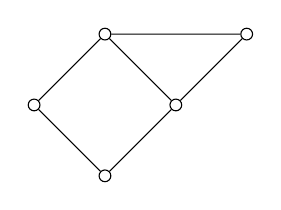
\begin{tikzpicture}[scale=.9]
    \foreach \i/\x/\y in {1/0/0,2/1/1,3/2/0,4/1/-1,5/3/1}
      \node[circle,draw,inner sep=1.5pt] (v\i) at (\x,\y) {};
    \draw (v1)--(v2)--(v3)--(v4)--(v1);
    \draw (v3)--(v5)--(v2);
  \end{tikzpicture}
  \begin{itemize}
    \item Use one small example before stating the general theorem.
    \item Ledger: record whether this is original, adapted, or source figure.
  \end{itemize}
\end{frame}

\begin{frame}{Main Bound Or Structure Theorem}
  \begin{theorem}
    State the extremal, enumeration, Ramsey, regularity, or probabilistic result.
  \end{theorem}
  \begin{itemize}
    \item Source: theorem number or paper section.
    \item Status: proved theorem, conjecture, sharp example, or heuristic.
    \item Ledger: record asymptotic regime and hidden constants.
  \end{itemize}
\end{frame}

\begin{frame}{Proof Method}
  \begin{enumerate}
    \item Counting, compression, induction, or polynomial method.
    \item Probabilistic, entropy, container, or regularity argument.
    \item Extremal construction or sharpness example.
  \end{enumerate}
\end{frame}
\end{document}
